\documentclass[11pt]{article}

\usepackage{iftex}
\ifPDFTeX
\usepackage[T1]{fontenc}
\usepackage[utf8]{inputenc}
\fi
\usepackage[margin=1in]{geometry}
\usepackage{amsmath, amssymb}
\usepackage{booktabs}
\usepackage[numbers]{natbib}
\usepackage{hyperref}
\usepackage{graphicx}
\usepackage{enumitem}
\usepackage{tikz}
\usetikzlibrary{arrows.meta, backgrounds, calc, fit, matrix, positioning}

\hypersetup{
  colorlinks=true,
  linkcolor=blue,
  citecolor=blue,
  urlcolor=blue
}

\title{KL-TE: Statistically Filtered Hierarchical Clustering with Projected Wald Tests}
\author{Draft workspace}
\date{\today}

\begin{document}

\maketitle

\begin{abstract}
A hierarchical tree proposes many candidate splits, but geometric tree cuts do
not say which of those splits are statistically credible. We describe KL-TE as
a statistically filtered hierarchical clustering method for binary,
categorical, and discretized continuous sample-feature data. The pipeline
builds an average-linkage Hamming tree on a working discrete representation,
assigns each internal node feature-wise distributions, and then answers the
node-level split question with two statistical tests. The child-parent edge
test asks whether at least one child departs from its ancestral context; it
uses nested variance, parent-local Marchenko--Pastur dimension selection,
eigenvalue whitening, and hierarchical Benjamini--Hochberg correction across
edges. The sibling test asks whether the two children are genuinely distinct
from one another; it uses Johnson--Lindenstrauss dimension selection and a
cousin-adjusted calibration model to deflate post-selection inflation before
Benjamini--Hochberg correction across focal sibling pairs. Categorical inputs
are handled through indicator expansion, while continuous inputs enter through
explicit discretization before the same tree-and-test pipeline is applied. The
corrected test annotations are converted into clusters by a top-down
pass-through traversal. This draft records the implemented method in its
present form and provides the mathematical description needed for the
empirical sections that still have to be added.
\end{abstract}

% !TEX root = ../main.tex

\section{Introduction}

Hierarchical clustering is attractive when the analyst wants more than a flat
partition. A tree exposes coarse-to-fine structure, keeps near-miss cluster
boundaries visible, and provides a natural substrate for interpretable cluster
decisions. In practice, however, most hierarchical
workflows still cut the tree using geometric heuristics such as a fixed height,
an inconsistency threshold, or a manually chosen number of clusters. Those
choices are often difficult to defend when the goal is not only descriptive
grouping but also reproducible statistical claims.

KL-TE takes a different view of the tree. An internal node is not merely a
merge artifact; it is a decision point. For a parent node $u$ with children
$l(u)$ and $r(u)$, the core question is: should this split survive in the final
partition? A linkage tree alone cannot answer that question. It proposes
candidate splits, but it does not tell us whether at least one child genuinely
departs from the parent's feature distribution, whether the two children are
actually distinct enough to represent separate clusters, or whether scanning
the entire tree has produced false positives.

The method therefore requires two kinds of evidence. First, a split should not
survive unless at least one child meaningfully departs from its ancestral
context. Second, even that is not enough: a parent can contain one drifting
branch or a mild asymmetry without supporting two stable child clusters, so the
children themselves must also be distinguishable from one another. This is why
the method uses both a child-parent edge test and a sibling test. The final
partition keeps a split only when both questions are answered favorably after
multiple-testing correction.

Four inferential complications shape the design. The child is a subset of its
parent, so the edge comparison is nested rather than an ordinary two-sample
test. The edge evidence is high-dimensional and correlated, so naive quadratic
aggregation would overcount redundant or noisy directions. Many candidate edges
are examined across the tree, so valid local $p$-values still require
multiplicity control. Finally, sibling comparisons are evaluated on a hierarchy
constructed from the same data, so the raw sibling statistics are selected and
inflated. The implemented method should be read as one response to these four
problems.

The implementation works on a discrete feature representation. Binary data
enter directly. Categorical data are represented through indicator-expanded
binary features. Continuous data are discretized before the same tree-and-test
pipeline is applied. Once the representation is fixed, the inferential objects
are no longer individual samples but subtrees, so each node carries a
feature-wise distribution estimated from its descendant leaves. Statistical
test annotations are computed before the actual tree walk that creates cluster
assignments. This separation between evidence calculation and final traversal
is useful both computationally and scientifically: the statistical support for
each potential split is stored explicitly and can be audited independently of
the resulting partition.

The manuscript follows that decision problem in order. It first constructs the
tree and node distributions that define the candidate splits. It then asks
whether a child departs from its parent, explains why that test needs nested
variance and spectral whitening, and applies hierarchical multiple-testing
control across the tree. It next asks whether the two children under the same
parent are genuinely distinct, and explains why that sibling comparison needs a
post-selection calibration step. Only after both evidence tables are in place
does the final tree traversal convert them into clusters.

At this stage the writing goal is to capture the statistical structure of the
method cleanly enough that the later experimental section can be attached
without rethinking the exposition. The immediate next step after this draft is
to add calibration and power studies that quantify when the inferential claims
made by these tests are empirically trustworthy.

% !TEX root = ../main.tex

\section{Method}

\subsection{Method overview}

The central question at every internal node can be stated directly: should this split
survive in the final partition? The hierarchy alone cannot answer it. A linkage
procedure proposes candidate splits, but it does not tell us whether a child
really leaves its parent's distributional background, whether the two children
are truly distinct from one another, or whether repeated testing across the
tree has created spurious evidence.

KL-TE answers that node-level question with two tests and one final traversal
rule. The child-parent edge test asks whether at least one branch departs from
its ancestral context. The sibling test asks whether the two children under the
same parent are distinct enough to justify keeping the split. Around those two
questions sit four practical complications that drive the rest of the method:
nested child-parent sampling, correlated high-dimensional edge evidence, many
tests across the tree, and post-selection inflation in sibling testing.

With that motivation in place, one full run of the method proceeds in the order
the code executes it:
\begin{enumerate}[leftmargin=1.5em]
  \item represent the input data in a discrete sample-feature matrix;
  \item build an average-linkage Hamming tree on the samples;
  \item assign every node a feature-wise distribution estimated from its
  descendant leaves;
  \item run the child-parent edge test on every parent-child edge to test
  whether a child subtree differs from its parent;
  \item run the sibling test on every binary sibling pair to test whether the two child
  subtrees are distinguishable from one another, then calibrate those sibling
  statistics for post-selection inflation;
  \item perform a top-down tree traversal that keeps a split only when the test
  annotations support it.
\end{enumerate}
The rest of this section follows that same logic rather than only the code
path. We first define the subtree-level objects being tested, then explain why
the child-parent comparison needs nested variance and spectral whitening, then
show why the sibling comparison requires a separate post-selection correction,
and finally describe how the resulting evidence tables are turned into
clusters.

\begin{figure}[p]
\centering
\vspace*{\fill}
\resizebox{\textwidth}{!}{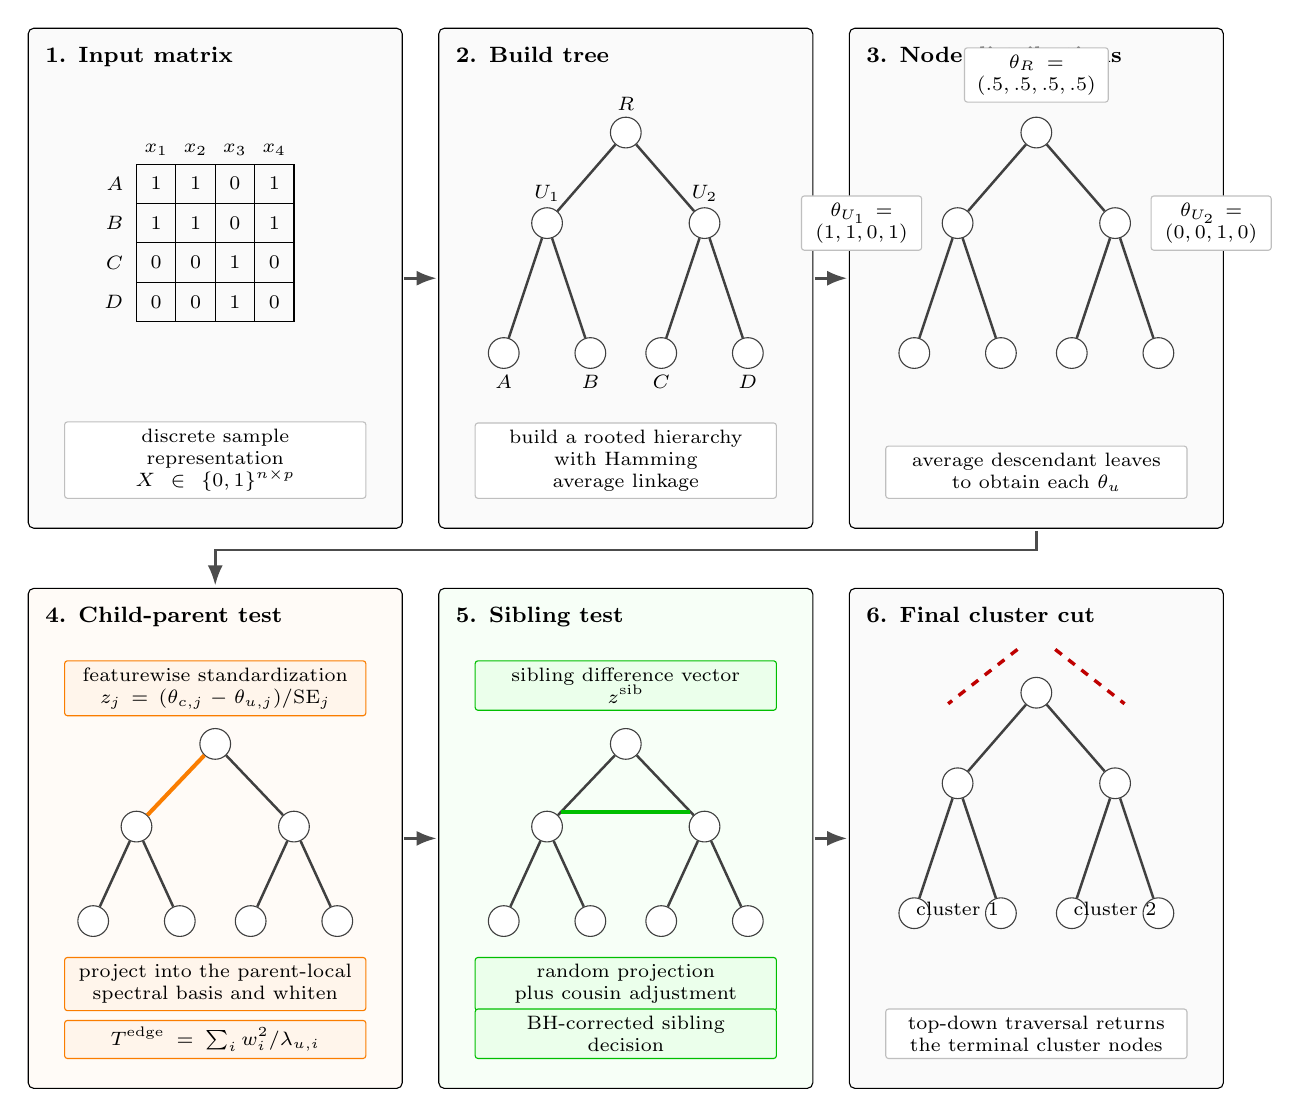
\begin{tikzpicture}[
  x=1cm,
  y=1cm,
  font=\small,
  >=Latex,
  panel/.style={
    draw,
    rounded corners=2pt,
    fill=gray!4,
    minimum width=4.75cm,
    minimum height=6.35cm,
    inner sep=5pt,
  },
  paneltitle/.style={font=\bfseries\footnotesize, anchor=north west},
  steparrow/.style={->, line width=0.95pt, draw=black!70},
  treeline/.style={line width=0.9pt, draw=black!75},
  gate2line/.style={draw=orange!98!black, line width=1.45pt},
  gate3line/.style={draw=green!75!black, line width=1.45pt},
  cutline/.style={draw=red!75!black, line width=1.25pt, dashed},
  treept/.style={circle, draw=black!75, fill=white, minimum size=3.9mm, inner sep=0pt},
  tinylabel/.style={font=\scriptsize, inner sep=1pt},
  eqbox/.style={
    draw=black!25,
    rounded corners=1pt,
    fill=white,
    inner sep=2.5pt,
    font=\scriptsize,
    align=center,
    text width=3.65cm,
  },
  gate2box/.style={eqbox, draw=orange!98!black, fill=orange!8},
  gate3box/.style={eqbox, draw=green!75!black, fill=green!8},
]

\node[panel] (p1) at (0,0) {};
\node[panel] (p2) [right=0.45cm of p1] {};
\node[panel] (p3) [right=0.45cm of p2] {};
\node[panel, fill=orange!3] (p4) [below=0.75cm of p1] {};
\node[panel, fill=green!3] (p5) [below=0.75cm of p2] {};
\node[panel] (p6) [below=0.75cm of p3] {};

\node[paneltitle] at ($(p1.north west)+(0.10,-0.12)$) {1. Input matrix};
\node[paneltitle] at ($(p2.north west)+(0.10,-0.12)$) {2. Build tree};
\node[paneltitle] at ($(p3.north west)+(0.10,-0.12)$) {3. Node distributions};
\node[paneltitle] at ($(p4.north west)+(0.10,-0.12)$) {4. Child-parent test};
\node[paneltitle] at ($(p5.north west)+(0.10,-0.12)$) {5. Sibling test};
\node[paneltitle] at ($(p6.north west)+(0.10,-0.12)$) {6. Final cluster cut};

% Panel 1
\matrix[
  matrix of nodes,
  nodes={draw, minimum width=0.50cm, minimum height=0.50cm, anchor=center, font=\scriptsize},
  row sep=-\pgflinewidth,
  column sep=-\pgflinewidth,
] (mat) at ($(p1.center)+(0,0.45)$) {
1 & 1 & 0 & 1 \\
1 & 1 & 0 & 1 \\
0 & 0 & 1 & 0 \\
0 & 0 & 1 & 0 \\
};
\node[tinylabel, anchor=east] at ($(mat-1-1.west)+(-0.12,0)$) {$A$};
\node[tinylabel, anchor=east] at ($(mat-2-1.west)+(-0.12,0)$) {$B$};
\node[tinylabel, anchor=east] at ($(mat-3-1.west)+(-0.12,0)$) {$C$};
\node[tinylabel, anchor=east] at ($(mat-4-1.west)+(-0.12,0)$) {$D$};
\foreach \c in {1,2,3,4} {
  \node[tinylabel, anchor=south] at ($(mat-1-\c.north)+(0,0.06)$) {$x_{\c}$};
}
\begin{scope}[on background layer]
  \fill[blue!10, rounded corners=1pt] ($(mat-1-1.north west)+(-0.04,0.04)$) rectangle ($(mat-2-4.south east)+(0.04,-0.04)$);
  \fill[blue!18, rounded corners=1pt] ($(mat-3-1.north west)+(-0.04,0.04)$) rectangle ($(mat-4-4.south east)+(0.04,-0.04)$);
\end{scope}
\node[eqbox, anchor=south] at ($(p1.south)+(0,0.38)$) {discrete sample representation\\$X \in \{0,1\}^{n \times p}$};

% Shared tree geometry macro via explicit coordinates
% Panel 2
\node[treept] (r2) at ($(p2.center)+(0,1.85)$) {};
\node[treept] (u21) at ($(p2.center)+(-1.00,0.70)$) {};
\node[treept] (u22) at ($(p2.center)+(1.00,0.70)$) {};
\node[treept] (a2) at ($(p2.center)+(-1.55,-0.95)$) {};
\node[treept] (b2) at ($(p2.center)+(-0.45,-0.95)$) {};
\node[treept] (c2) at ($(p2.center)+(0.45,-0.95)$) {};
\node[treept] (d2) at ($(p2.center)+(1.55,-0.95)$) {};
\draw[treeline] (r2) -- (u21);
\draw[treeline] (r2) -- (u22);
\draw[treeline] (u21) -- (a2);
\draw[treeline] (u21) -- (b2);
\draw[treeline] (u22) -- (c2);
\draw[treeline] (u22) -- (d2);
\node[tinylabel, above=1pt of r2] {$R$};
\node[tinylabel, above=1pt of u21] {$U_1$};
\node[tinylabel, above=1pt of u22] {$U_2$};
\node[tinylabel, below=1pt of a2] {$A$};
\node[tinylabel, below=1pt of b2] {$B$};
\node[tinylabel, below=1pt of c2] {$C$};
\node[tinylabel, below=1pt of d2] {$D$};
\node[eqbox, anchor=south] at ($(p2.south)+(0,0.38)$) {build a rooted hierarchy\\with Hamming average linkage};

% Panel 3
\node[treept] (r3) at ($(p3.center)+(0,1.85)$) {};
\node[treept] (u31) at ($(p3.center)+(-1.00,0.70)$) {};
\node[treept] (u32) at ($(p3.center)+(1.00,0.70)$) {};
\node[treept] (a3) at ($(p3.center)+(-1.55,-0.95)$) {};
\node[treept] (b3) at ($(p3.center)+(-0.45,-0.95)$) {};
\node[treept] (c3) at ($(p3.center)+(0.45,-0.95)$) {};
\node[treept] (d3) at ($(p3.center)+(1.55,-0.95)$) {};
\draw[treeline] (r3) -- (u31);
\draw[treeline] (r3) -- (u32);
\draw[treeline] (u31) -- (a3);
\draw[treeline] (u31) -- (b3);
\draw[treeline] (u32) -- (c3);
\draw[treeline] (u32) -- (d3);
\node[eqbox, text width=1.65cm, anchor=south] at ($(r3)+(0,0.38)$) {$\theta_R=$\\$(.5,.5,.5,.5)$};
\node[eqbox, text width=1.35cm, anchor=east] at ($(p3.center)+(-1.45,0.70)$) {$\theta_{U_1}=$\\$(1,1,0,1)$};
\node[eqbox, text width=1.35cm, anchor=west] at ($(p3.center)+(1.45,0.70)$) {$\theta_{U_2}=$\\$(0,0,1,0)$};
\node[eqbox, anchor=south] at ($(p3.south)+(0,0.38)$) {average descendant leaves\\to obtain each $\theta_u$};

% Panel 4
\node[treept] (r4) at ($(p4.center)+(0,1.20)$) {};
\node[treept] (u41) at ($(p4.center)+(-1.00,0.15)$) {};
\node[treept] (u42) at ($(p4.center)+(1.00,0.15)$) {};
\node[treept] (a4) at ($(p4.center)+(-1.55,-1.05)$) {};
\node[treept] (b4) at ($(p4.center)+(-0.45,-1.05)$) {};
\node[treept] (c4) at ($(p4.center)+(0.45,-1.05)$) {};
\node[treept] (d4) at ($(p4.center)+(1.55,-1.05)$) {};
\draw[treeline] (r4) -- (u41);
\draw[treeline] (r4) -- (u42);
\draw[treeline] (u41) -- (a4);
\draw[treeline] (u41) -- (b4);
\draw[treeline] (u42) -- (c4);
\draw[treeline] (u42) -- (d4);
\draw[gate2line] (r4) -- (u41);
\node[gate2box, anchor=north] at ($(p4.north)+(0,-0.92)$) {featurewise standardization\\$z_j=(\theta_{c,j}-\theta_{u,j})/\mathrm{SE}_j$};
\node[gate2box] at ($(p4.center)+(0,-1.85)$) {project into the parent-local\\spectral basis and whiten};
\node[gate2box, anchor=south] at ($(p4.south)+(0,0.38)$) {$T^{\mathrm{edge}}=\sum_i w_i^2/\lambda_{u,i}$};

% Panel 5
\node[treept] (r5) at ($(p5.center)+(0,1.20)$) {};
\node[treept] (u51) at ($(p5.center)+(-1.00,0.15)$) {};
\node[treept] (u52) at ($(p5.center)+(1.00,0.15)$) {};
\node[treept] (a5) at ($(p5.center)+(-1.55,-1.05)$) {};
\node[treept] (b5) at ($(p5.center)+(-0.45,-1.05)$) {};
\node[treept] (c5) at ($(p5.center)+(0.45,-1.05)$) {};
\node[treept] (d5) at ($(p5.center)+(1.55,-1.05)$) {};
\draw[treeline] (r5) -- (u51);
\draw[treeline] (r5) -- (u52);
\draw[treeline] (u51) -- (a5);
\draw[treeline] (u51) -- (b5);
\draw[treeline] (u52) -- (c5);
\draw[treeline] (u52) -- (d5);
\draw[gate3line] ($(u51)+(0.18,0.18)$) -- ($(u52)+(-0.18,0.18)$);
\node[gate3box, anchor=north] at ($(p5.north)+(0,-0.92)$) {sibling difference vector\\$z^{\mathrm{sib}}$};
\node[gate3box] at ($(p5.center)+(0,-1.85)$) {random projection\\plus cousin adjustment};
\node[gate3box, anchor=south] at ($(p5.south)+(0,0.38)$) {BH-corrected sibling\\decision};

% Panel 6
\node[treept] (r6) at ($(p6.center)+(0,1.85)$) {};
\node[treept] (u61) at ($(p6.center)+(-1.00,0.70)$) {};
\node[treept] (u62) at ($(p6.center)+(1.00,0.70)$) {};
\node[treept] (a6) at ($(p6.center)+(-1.55,-0.95)$) {};
\node[treept] (b6) at ($(p6.center)+(-0.45,-0.95)$) {};
\node[treept] (c6) at ($(p6.center)+(0.45,-0.95)$) {};
\node[treept] (d6) at ($(p6.center)+(1.55,-0.95)$) {};
\draw[treeline] (r6) -- (u61);
\draw[treeline] (r6) -- (u62);
\draw[treeline] (u61) -- (a6);
\draw[treeline] (u61) -- (b6);
\draw[treeline] (u62) -- (c6);
\draw[treeline] (u62) -- (d6);
\draw[cutline] ($(r6)+(-0.24,0.55)$) -- ($(r6)+(-1.12,-0.14)$);
\draw[cutline] ($(r6)+(0.24,0.55)$) -- ($(r6)+(1.12,-0.14)$);
\begin{scope}[on background layer]
  \fill[blue!10, rounded corners=2pt] ($(u61)+(-0.72,-1.32)$) rectangle ($(u61)+(0.72,0.35)$);
  \fill[green!10, rounded corners=2pt] ($(u62)+(-0.72,-1.32)$) rectangle ($(u62)+(0.72,0.35)$);
\end{scope}
\node[tinylabel, anchor=north] at ($(u61)+(0,-1.46)$) {cluster 1};
\node[tinylabel, anchor=north] at ($(u62)+(0,-1.46)$) {cluster 2};
\node[eqbox, anchor=south] at ($(p6.south)+(0,0.38)$) {top-down traversal returns\\the terminal cluster nodes};

\draw[steparrow] ($(p1.east)+(0.02,0)$) -- ($(p2.west)+(-0.02,0)$);
\draw[steparrow] ($(p2.east)+(0.02,0)$) -- ($(p3.west)+(-0.02,0)$);
\draw[steparrow] ($(p3.south)+(0,-0.03)$) -- ++(0,-0.24) -| ($(p4.north)+(0.00,0.03)$);
\draw[steparrow] ($(p4.east)+(0.02,0)$) -- ($(p5.west)+(-0.02,0)$);
\draw[steparrow] ($(p5.east)+(0.02,0)$) -- ($(p6.west)+(-0.02,0)$);

\end{tikzpicture}
}
\caption{Pedagogical overview of one full KL-TE run. The panels correspond to
the successive requirements in the split decision: represent the data, build a
tree of candidate splits, summarize each subtree by a node distribution, test
whether a child departs from its parent, test whether the two children are
genuinely distinct, and only then keep the split in the final top-down
traversal. The figure is schematic: it shows why each stage is needed, not just
the order in which the code executes it.}
\label{fig:pipeline-overview}
\vspace*{\fill}
\end{figure}

\subsection{Representation, tree construction, and node distributions}

Let $X$ denote the working sample representation after any preprocessing. In
the direct binary or indicator case,
$X \in \{0,1\}^{n \times p}$ with rows $X_i \in \{0,1\}^p$. Categorical and
continuous inputs are mapped into this same discrete representation before the
tree is built. The method builds a rooted agglomerative tree
$\mathcal{T} = (V,E)$ using Hamming distance between samples and average
linkage. Leaves are in one-to-one correspondence with the original samples.

Once that tree is fixed, the inferential problem is about subtrees rather than
individual samples. The method therefore replaces each node by an empirical
feature distribution over its descendant leaves. This is the object that enters
both tests: the edge test compares a child distribution to its parent's
distribution, and the sibling test compares the two child distributions under
the same parent. The raw leaf matrix still matters through the descendant sets
and local spectral matrices, but the primary inferential units are node-level
distributions.

For each node $u \in V$, let $L(u)$ denote its descendant leaf set and let
$n_u = |L(u)|$. For binary or indicator coordinates, the node distribution is
the feature-wise mean vector
\begin{equation}
\theta_u = \frac{1}{n_u}\sum_{i \in L(u)} X_i \in [0,1]^p.
\end{equation}
If $u$ has children $l$ and $r$, then
\begin{equation}
n_u = n_l + n_r,
\qquad
\theta_u = \frac{n_l \theta_l + n_r \theta_r}{n_u}.
\end{equation}
The decomposition goal is to identify a set of terminal tree nodes whose leaf
sets partition the samples and whose defining splits are supported by the two
statistical tests below. These formulas cover binary data directly and also the
indicator representations used for categorical and discretized continuous data.

Categorical features with values $C_{ij} \in \{0,\dots,K-1\}$ are represented
through one-hot indicators
\begin{equation}
\tilde{X}_{i,j,k} = \mathbf{1}\{C_{ij} = k\},
\qquad
k = 0,\dots,K-1,
\end{equation}
so that the Bernoulli/indicator formulas below apply directly on the expanded
feature space. Continuous inputs enter through an explicit preprocessing map
into a discrete representation. Median binarization is
\begin{equation}
X_{ij}^{\mathrm{bin}}
=
\mathbf{1}\!\left\{
W_{ij} > \mathrm{median}(W_{\cdot j})
\right\},
\end{equation}
and quantile discretization followed by one-hot expansion is
\begin{equation}
C_{ij}
=
\sum_{q=1}^{K-1} \mathbf{1}\{W_{ij} > t_{jq}\},
\qquad
t_{jq} = Q_{q/K}(W_{\cdot j}),
\end{equation}
with the same indicator map
$\tilde{X}_{i,j,k} = \mathbf{1}\{C_{ij} = k\}$. After this representation step,
the same tree construction and testing logic are used for all supported input
types.

\subsection{Child-parent edge test}

The child-parent edge test is the first inferential step. For each edge
$(u,c) \in E$, it asks whether child $c$ carries signal beyond its parent $u$.
This is the method's first guard against keeping a split just because the
linkage algorithm happened to create one. In plain terms, the question is:
does this child really move away from the background defined by its parent, or
is the observed difference small enough to be explained by sampling noise?

The raw difference $\theta_c-\theta_u$ is not enough on its own. Some features
are naturally more variable than others, and very small child subtrees are
noisier than large ones. The test therefore begins by converting the raw
child-parent difference into standardized feature scores. The coordinate-wise null is
$H_{0,j}^{\mathrm{edge}}(u,c): \theta_{c,j} = \theta_{u,j}$. Because $c$ is
nested inside $u$, the child and parent estimators are not independent. In the
binary or indicator representation,
\begin{equation}
\mathrm{Var}(\hat{\theta}_{c,j} - \hat{\theta}_{u,j})
=
\theta_{u,j}(1-\theta_{u,j})
\left(\frac{1}{n_c} - \frac{1}{n_u}\right),
\end{equation}
which is the variance expression used in the code. The standardized edge vector
is therefore
\begin{equation}
z_{u \to c,j}^{\mathrm{edge}}
=
\frac{\theta_{c,j} - \theta_{u,j}}
{\sqrt{\theta_{u,j}(1-\theta_{u,j})\left(\frac{1}{n_c} - \frac{1}{n_u}\right)}}.
\end{equation}
This standardization is applied \emph{coordinatewise}. Each feature first gets
its own z-like score before the method combines evidence across features. For a
parent-child edge with $p$ binary or indicator coordinates, the implementation first computes $p$ scalar standardized scores
$z_{u \to c,1}^{\mathrm{edge}},\dots,z_{u \to c,p}^{\mathrm{edge}}$, one for
each feature, then stacks them into the vector
\begin{equation}
z_{u \to c}^{\mathrm{edge}}
=
\left(
z_{u \to c,1}^{\mathrm{edge}},
\dots,
z_{u \to c,p}^{\mathrm{edge}}
\right)^\top
\in \mathbb{R}^p.
\end{equation}
The subtraction term
$\frac{1}{n_c} - \frac{1}{n_u}$ is the signature of the nested tree setting.
In an ordinary two-sample test for independent groups, the variance factor
would look like $\frac{1}{n_1} + \frac{1}{n_2}$. Here the parent already
contains the child, so part of the uncertainty cancels out, which yields the
nested factor $\frac{1}{n_c} - \frac{1}{n_u} > 0$. This is why very small
children need a larger raw deviation $\theta_{c,j} - \theta_{u,j}$ to generate
the same standardized score.

Coordinatewise standardization fixes heteroskedasticity, but it does not solve
the second problem: the edge evidence is high-dimensional and correlated.
Summing $z_{u \to c,j}^2$ directly would overcount redundant coordinates and let
noisy directions dominate just because they contribute many small correlated
terms. The method therefore looks for a smaller set of parent-local directions
that summarize the main variation seen below the parent, and it measures the
edge deviation in that reduced space. For each parent node $u$, the
implementation forms a local matrix $M_u$ whose rows are:
\begin{enumerate}[leftmargin=1.5em]
  \item all descendant leaf vectors $X_i$ for $i \in L(u)$, and
  \item all descendant internal-node distributions $\theta_v$ for proper
  descendants $v$ of $u$.
\end{enumerate}
After removing constant features, let $d_u$ be the number of active
coordinates and let $m_u$ be the number of rows in $M_u$. The code computes the correlation matrix
$C_u \in \mathbb{R}^{d_u \times d_u}$ and its eigen-decomposition
\begin{equation}
C_u = V_u \Lambda_u V_u^\top,
\qquad
\Lambda_u = \mathrm{diag}(\lambda_{u,1},\dots,\lambda_{u,d_u}),
\qquad
\lambda_{u,1} \ge \cdots \ge \lambda_{u,d_u} \ge 0.
\end{equation}
Equivalently, if $\widetilde{M}_u \in \mathbb{R}^{m_u \times d_u}$ denotes the
column-standardized active-coordinate submatrix of $M_u$ after centering each
active feature to mean zero and scaling it to unit variance, then
\begin{equation}
C_u = \frac{1}{m_u}\widetilde{M}_u^\top \widetilde{M}_u,
\end{equation}
up to the standard Pearson-correlation normalization already enforced by the
column standardization. In practice, this matrix identifies the main patterns
of co-variation visible below the parent. When $m_u < d_u$, the implementation
switches to the dual standardized Gram matrix
\begin{equation}
G_u = \frac{1}{d_u}\widetilde{M}_u \widetilde{M}_u^\top,
\end{equation}
whose nonzero eigenvalues coincide with those of $C_u$, so the same local
summary is recovered in a computationally cheaper form.

The spectral dimension is the Marchenko--Pastur signal count
\citep{marchenko1967distribution}. With
\begin{equation}
\hat{\sigma}_u^2 = \mathrm{median}\{\lambda_{u,i} : \lambda_{u,i} > 0\},
\qquad
b_u^{\mathrm{MP}} = \hat{\sigma}_u^2 \left(1 + \sqrt{\frac{d_u}{m_u}}\right)^2,
\end{equation}
the projection dimension is
\begin{equation}
k_u^{\mathrm{edge}}
=
\max\left\{
2,\;
\#\{i : \lambda_{u,i} > b_u^{\mathrm{MP}}\}
\right\},
\end{equation}
followed by the implementation cap $k_u^{\mathrm{edge}} \le d_u$. The floor is
$2$.

Let $v_{u,1},\dots,v_{u,k_u^{\mathrm{edge}}}$ denote the leading eigenvectors.
After the coordinatewise standardization step, the vector
$z_{u \to c}^{\mathrm{edge}} \in \mathbb{R}^p$ is projected onto these
parent-local directions. The edge test then rescales those projected
coordinates so that noisy directions do not automatically count more than
stable ones. The resulting test statistic is
\begin{equation}
T_{u \to c}^{\mathrm{edge}}
=
\sum_{i=1}^{k_u^{\mathrm{edge}}}
\frac{(v_{u,i}^\top z_{u \to c}^{\mathrm{edge}})^2}{\lambda_{u,i}}.
\end{equation}
Writing
$w_{u \to c,i} = v_{u,i}^\top z_{u \to c}^{\mathrm{edge}}$ for the projected
coordinate along the $i$th parent-local spectral direction, each summand is
\begin{equation}
\frac{w_{u \to c,i}^2}{\lambda_{u,i}}.
\end{equation}
This is the practical role of the projection-and-whitening step. The projection
rewrites the edge deviation in directions that are actually present in the
subtree below $u$, and the whitening step stops high-variance background
directions from dominating the test merely because they are noisy.
Under the local correlation-model approximation used by the implementation, the
resulting statistic is calibrated against a $\chi^2_{k_u^{\mathrm{edge}}}$
reference law:
\begin{equation}
T_{u \to c}^{\mathrm{edge}} \sim \chi^2_{k_u^{\mathrm{edge}}},
\qquad
p_{u \to c}^{\mathrm{edge}}
=
\Pr\!\left(
\chi^2_{k_u^{\mathrm{edge}}}
\ge
T_{u \to c}^{\mathrm{edge}}
\right).
\end{equation}
This calibration is exact in the pure PCA-whitened case. In the implemented
mixed-basis path, if fewer usable PCA directions are available than the
nominal target dimension, the implementation simply uses the available
parent-local rows rather than padding with unrelated random directions.
\paragraph{Worked child-parent example.}
The worked example below is intended to show the logic of the edge test, not
just the algebra. It starts with a parent-child comparison that is visibly
different by eye, then shows how each formula answers one of the two problems
above: nested variance and correlated high-dimensional evidence. Consider four
binary samples
\begin{equation}
A=(1,1,0,1),\quad
B=(1,1,0,1),\quad
C=(0,0,1,0),\quad
D=(0,0,1,0),
\end{equation}
with tree root $R$ and children $U_1=\{A,B\}$ and $U_2=\{C,D\}$. The node
distributions are
\begin{equation}
\theta_{U_1}=(1,1,0,1),\qquad
\theta_{U_2}=(0,0,1,0),\qquad
\theta_R=(0.5,0.5,0.5,0.5).
\end{equation}
Because the implementation includes proper descendant internal distributions in
the spectral matrix, the root-local matrix is
\begin{equation}
M_R =
\begin{bmatrix}
1&1&0&1\\
1&1&0&1\\
0&0&1&0\\
0&0&1&0\\
1&1&0&1\\
0&0&1&0
\end{bmatrix},
\end{equation}
where the first four rows are the leaves $A,B,C,D$ and the last two rows are
the internal-node distributions $\theta_{U_1}$ and $\theta_{U_2}$. Each active
column has mean $0.5$ and standard deviation $0.5$, so the standardized matrix
is
\begin{equation}
\widetilde{M}_R =
\begin{bmatrix}
1&1&-1&1\\
1&1&-1&1\\
-1&-1&1&-1\\
-1&-1&1&-1\\
1&1&-1&1\\
-1&-1&1&-1
\end{bmatrix}.
\end{equation}
The corresponding parent-local correlation matrix is
\begin{equation}
C_R =
\begin{bmatrix}
1&1&-1&1\\
1&1&-1&1\\
-1&-1&1&-1\\
1&1&-1&1
\end{bmatrix},
\end{equation}
whose eigenvalues are
\begin{equation}
(\lambda_{R,1},\lambda_{R,2},\lambda_{R,3},\lambda_{R,4}) = (4,0,0,0).
\end{equation}
One leading eigenvector is
\begin{equation}
v_{R,1} = (0.5,0.5,-0.5,0.5)^\top.
\end{equation}
Now test the edge $R \to U_1$. Since $n_R=4$ and $n_{U_1}=2$, the nested
variance factor is
\begin{equation}
\frac{1}{n_{U_1}} - \frac{1}{n_R} = \frac{1}{2} - \frac{1}{4} = \frac{1}{4}.
\end{equation}
Because each root coordinate equals $0.5$, every feature has variance
\begin{equation}
0.5(1-0.5)\left(\frac{1}{2}-\frac{1}{4}\right)=0.0625.
\end{equation}
Using the coordinatewise standardization formula above, the edge vector is
\begin{equation}
z_{R \to U_1}^{\mathrm{edge}}
=
\frac{(1,1,0,1)-(0.5,0.5,0.5,0.5)}{\sqrt{0.0625}}
=
(2,2,-2,2)^\top.
\end{equation}
Projecting onto the leading spectral direction gives
\begin{equation}
w_{R \to U_1,1}
=
v_{R,1}^\top z_{R \to U_1}^{\mathrm{edge}}
=
0.5\cdot 2 + 0.5\cdot 2 - 0.5\cdot (-2) + 0.5\cdot 2
=
4.
\end{equation}
Therefore the first whitened contribution to the edge-test statistic is
\begin{equation}
\frac{w_{R \to U_1,1}^2}{\lambda_{R,1}}
=
\frac{4^2}{4}
=
4.
\end{equation}
This example shows the full logic of the child-parent edge test in the same
order as the formulas: standardize the raw difference, express it in the main
parent-level directions, and then down-weight directions that are mostly noise.
In larger real subtrees the implementation can use more than one such
direction, but the core interpretation is already visible in this toy example.
These $p$-values are computed for every edge in the tree.

\subsection{Hierarchical multiple testing across edges}

Even a well-calibrated edge test would over-split the hierarchy if it were
applied independently to every edge and thresholded at a fixed level. The tree
contains many overlapping candidate splits, and the final partition depends on
reading those edge decisions jointly. The method therefore applies a
hierarchical Benjamini--Hochberg correction on the tree
\citep{bogomolov2021hypotheses} at level
$\alpha_{\mathrm{edge}} = 0.001$. Edge hypotheses are grouped into families by
parent node. If $F(u)$ denotes the family of edges from parent $u$ to its
children, then the family-specific level used by the implementation is
\begin{equation}
\alpha_u
=
\alpha_{\mathrm{edge}}
\prod_{a \in \mathrm{Anc}(u)}
\frac{R_a}{|F(a)|},
\end{equation}
where $R_a$ is the number of rejections already made in the ancestor family
$F(a)$. Intuitively, evidence is allowed to propagate downward only after
earlier parts of the tree have already shown signal. Root families start at
$\alpha_{\mathrm{edge}}$. Within each family, ordinary Benjamini--Hochberg is
applied at level $\alpha_u$. Let
$S^{\mathrm{edge}}(c) \in \{0,1\}$ denote the resulting significance indicator
for child $c$.

\subsection{Sibling test with post-selection adjustment}

The sibling test is the second inferential step. For each parent $u$ with
exactly two children $l(u)$ and $r(u)$, it asks whether the two children are
genuinely different from one another rather than merely both differing from the
parent. The edge test alone is not enough to justify keeping a split. A parent
can contain one deviating branch, or a weak left-right asymmetry, without
supporting two stable child clusters. The sibling test supplies that missing
question: once a branch has left its ancestral context, are the two children
actually distinct enough to become separate clusters?
Formally, it tests the sibling null
\begin{equation}
H_0^{\mathrm{sib}}(u): \theta_{l(u)} = \theta_{r(u)}.
\end{equation}
For binary or indicator coordinates, the pooled null proportion is
\begin{equation}
\bar{\theta}_{u,j}
=
\frac{n_{l(u)}\theta_{l(u),j} + n_{r(u)}\theta_{r(u),j}}
{n_{l(u)} + n_{r(u)}}.
\end{equation}
The standardized sibling vector is
\begin{equation}
z_{u,j}^{\mathrm{sib}}
=
\frac{\theta_{l(u),j} - \theta_{r(u),j}}
{\sqrt{
\bar{\theta}_{u,j}(1-\bar{\theta}_{u,j})
\left(\frac{1}{n_{l(u)}} + \frac{1}{n_{r(u)}}\right)
}}.
\end{equation}
The sibling test then asks how to combine this multi-feature contrast into one
summary score. Unlike older versions of the method, the current implementation
does not choose a fresh random projection here. Instead it reuses the spectral
information already computed during the child-parent stage. For a binary
parent $u$ with children $l(u)$ and
$r(u)$, let $k_{l(u)}^{\mathrm{edge}}$ and $k_{r(u)}^{\mathrm{edge}}$ denote
the positive edge-stage spectral dimensions of the two children. The sibling
dimension is then
\begin{equation}
k_u^{\mathrm{sib}}
=
\min\left\{
k_{l(u)}^{\mathrm{edge}},\; k_{r(u)}^{\mathrm{edge}}
\right\}
\end{equation}
after excluding any child with zero detected signal dimension. This
deliberately conservative rule means that a sibling split is judged only in
dimensions that both child subtrees appear to support. If neither child has a
positive edge-stage dimension, the sibling test is skipped and the node is
treated conservatively as a merge.

The projection basis itself comes from the parent node, not from a random draw.
This choice is easier to interpret for the reader and the analyst: the parent
PCA directions summarize the dominant axes of variation visible at the level
where the sibling split is being judged. In the common case, the first
$k_u^{\mathrm{sib}}$ parent PCA directions are used directly. When the
requested sibling dimension exceeds the number of usable parent directions, the
implementation may append additional directions taken from the parts of the
child PCA spaces that are orthogonal to the parent basis. If such extra
directions are unavailable, the test simply uses the parent directions that
exist.

If $P_u \in \mathbb{R}^{k_u^{\mathrm{sib}} \times p}$ denotes this sibling
projection basis, the raw sibling statistic is
\begin{equation}
T_u^{\mathrm{raw}}
=
\|P_u z_u^{\mathrm{sib}}\|_2^2.
\end{equation}
The default p-value calculation is deliberately conservative. After
projection, the method asks whether the observed squared contrast is larger
than would be expected from ordinary within-parent sampling noise, while still
allowing different projected directions to have different variances. In the
current implementation, this is done with a Satterthwaite moment match for the
PCA-derived part of the test and plain $\chi^2(1)$ contributions for any added
orthogonal-complement directions.

Raw sibling $p$-values are still not enough on their own. The same data are
used to build the hierarchy, choose which nodes matter, and evaluate sibling
contrasts. That reuse creates \emph{post-selection inflation}: the tree has
already been optimized to separate the data, so the observed sibling
difference vector $z_u^{\mathrm{sib}}$ is systematically larger than it would
be under a fresh null sample, even when the data contain no cluster structure.
Empirical null simulations confirm that the uncorrected Wald sibling test
produces Type~I error rates of approximately 39\% at $\alpha = 0.05$.

\paragraph{Calibration via continuous edge-weight deflation.}
The sibling calibration then corrects for this extra optimism by estimating one
global adjustment factor $\hat{c}$ from the sibling statistics themselves,
using the edge-test $p$-values as continuous weights. Intuitively, sibling
pairs that already look noisy receive more weight when estimating the
correction, while pairs that look strongly structured receive less. For every
parent $q$ with exactly two children, define the inflation ratio
\begin{equation}
r_q = \frac{T_q^{\mathrm{raw}}}{k_q^{\mathrm{sib}}}.
\end{equation}
Under $H_0$, each component of the projected difference is approximately
$\mathcal{N}(0,c)$ with $c > 1$ reflecting post-selection inflation, so
$\mathbb{E}[r_q] = c$.  The key idea is to weight each pair by how likely it
is to be a genuine null:
\begin{equation}
w_q = \min\!\left(p^{\mathrm{edge}}_{l(q)},\;
                    p^{\mathrm{edge}}_{r(q)}\right),
\end{equation}
where $p^{\mathrm{edge}}_{l(q)}$ and $p^{\mathrm{edge}}_{r(q)}$ are the
BH-corrected edge-test $p$-values of the two children. Pairs where neither
child is edge-significant receive large weights and dominate the estimate,
while pairs with genuine cluster signal receive small weights and are
effectively down-weighted. The global inflation factor is then the
weighted mean
\begin{equation}\label{eq:chat-global}
\hat{c}
=
\frac{\sum_q w_q \, r_q}{\sum_q w_q},
\qquad
\text{clamped to } [1,\;\max_q r_q].
\end{equation}

\paragraph{Why continuous weights, not a binary oracle.}
An earlier design classified sibling pairs into discrete \emph{null-like}
(neither child edge-significant) and \emph{focal} groups, then fitted the
calibration model only on null-like pairs.  This approach has a circular
dependency: on null data, the edge test itself is inflated by post-selection
bias and declares essentially every edge significant---leaving zero null-like
calibration pairs and forcing $\hat{c}=1$ (no correction).  Empirical tracing
on pure-noise data ($n=100$, $p=50$, $K_{\mathrm{true}}=1$) confirmed this
failure: the edge test marked 198 of 199 edges significant, the calibration
received zero null-like pairs, and the method returned $K=17$. Continuous
weighting avoids this dead zone: even when all edge $p$-values are similarly
small, the weights are approximately equal, and the weighted mean of $r_q$
still recovers the true inflation $\hat{c} \approx 3$.

\paragraph{Single global correction.}
The current implementation uses one global correction rather than a different
correction at every node. This keeps the adjustment simple, avoids unstable
extrapolation at large nodes, and separates the question of post-selection bias
from the separate question of how strong the signal is in a particular part of
the tree.

For each focal pair $u$, the adjusted sibling test is
\begin{equation}
T_u^{\mathrm{adj}} = \frac{T_u^{\mathrm{raw}}}{\hat{c}},
\qquad
p_u^{\mathrm{sib}}
=
\Pr\!\left(\widetilde{\chi}^2_u \ge T_u^{\mathrm{adj}}\right),
\end{equation}
where $\widetilde{\chi}^2_u$ denotes the same sibling reference law used for the
raw test: by default, the Satterthwaite moment match induced by the parent PCA
eigenvalues and any added padding directions.
This is a practical calibration model for post-selection inflation, not a
separate finite-sample exact theorem for the adjusted sibling statistic.

The sibling multiplicity correction is ordinary
Benjamini--Hochberg \citep{benjamini1995controlling} at
$\alpha_{\mathrm{sib}} = 0.01$, applied only across focal sibling pairs. Let
$S^{\mathrm{sib}}(u) \in \{0,1\}$ denote the resulting indicator that parent
$u$ supports a significant sibling split.

\subsection{Recursive decomposition rule}

Once the edge-test and sibling-test annotations are available, the inferential
work is finished. The remaining step is purely algorithmic: traverse the tree
from the root downward and decide where the splits are kept. The traversal does
not estimate any new model or compute any new $p$-values; it turns the
precomputed evidence tables into a final partition.

The final clusters are produced by a top-down traversal that reads the two test
annotation tables. For an internal node $u$ with children $l(u)$ and $r(u)$,
the split rule is
\begin{equation}
\mathrm{Split}(u) = 1
\end{equation}
if and only if all three conditions hold:
\begin{enumerate}[leftmargin=1.5em]
  \item $u$ has exactly two children;
  \item $S^{\mathrm{edge}}(l(u)) = 1$ or $S^{\mathrm{edge}}(r(u)) = 1$;
  \item $S^{\mathrm{sib}}(u) = 1$.
\end{enumerate}
If these conditions hold, traversal continues into both children. Otherwise the
method would ordinarily stop and declare $u$ a terminal cluster.

However, the implementation also enables pass-through traversal. Let
$D^{\mathrm{sib}}(u)$ be the indicator that some proper descendant of $u$ has a
significant non-skipped sibling split. Then the traversal still descends into
both children when
\begin{equation}
\mathrm{Split}(u) = 0,
\qquad
u \text{ has exactly two children},
\qquad
S^{\mathrm{edge}}(l(u)) \vee S^{\mathrm{edge}}(r(u)) = 1,
\qquad
D^{\mathrm{sib}}(u) = 1.
\end{equation}
This is the pass-through rule used to prevent a shallow sibling-test failure from
masking deeper structure. The terminal nodes returned by this traversal define
the final cluster partition directly.

% !TEX root = ../main.tex

\section{Practical Setup}

Table~\ref{tab:defaults} summarizes the main settings used in the current
implementation. These settings define how the tree is built, how evidence is
combined across the tree, and how final cluster decisions are made.

\begin{table}[ht]
\centering
\begin{tabular}{ll}
\toprule
Component & Current choice \\
\midrule
Tree distance & Hamming \\
Linkage & Average linkage \\
Edge significance level & $\alpha_{\mathrm{edge}} = 0.001$ \\
Sibling significance level & $\alpha_{\mathrm{sib}} = 0.01$ \\
Edge test & Projected Wald test with parent-specific whitening \\
Edge dimension rule & Signal count from the parent's local spectrum \\
Sibling test & Projected Wald test with edge-weight adjustment \\
Sibling dimension rule & Smallest positive child signal dimension \\
Sibling basis / calibration & Parent PCA basis, Satterthwaite default \\
Minimum spectral dimension & 2 \\
Include internal spectral rows & On \\
Edge multiple-testing correction & Hierarchical BH correction on the tree \\
Sibling multiple-testing correction & Flat BH on focal pairs \\
Pass-through traversal & On \\
\bottomrule
\end{tabular}
\caption{Main settings used in the current implementation.}
\label{tab:defaults}
\end{table}

Two aspects of the setup deserve special emphasis. First, the two tests do not
combine information in the same way. The child-parent edge test asks whether a
child leaves the background defined by its parent. The sibling test then asks
whether the two children are different enough from one another to justify
keeping the split. Second, once those test tables exist, the final clustering
step is simple: the method walks down the tree and keeps only the splits that
remain supported after correction.

The representation layer should also be read as part of the method. Binary data
enter directly, categorical data enter through one-hot indicator expansion, and
continuous data are discretized before the same testing procedure is applied.

\section{Experimental Plan}

This section is a forward-looking placeholder. Before the method can support
publication-quality inferential claims, the manuscript should cover at least
the following empirical blocks.

\subsection{Null calibration}

The first requirement is a null calibration study on binary data with no true
cluster structure. The goal is to measure how often Gate 2 and Gate 3 reject
under scenarios where they should not. This should be reported both at the
individual-test level and at the resulting number-of-clusters level. The latter
is critical because a method can have mild per-test inflation yet still produce
severe over-splitting once the tree walk is applied.

\subsection{Power under planted structure}

The second requirement is a controlled power study with planted binary subtrees.
This should vary:

\begin{itemize}[leftmargin=1.5em]
  \item sample size per cluster,
  \item effect size in feature rates,
  \item number of informative features,
  \item tree imbalance, and
  \item background noise level.
\end{itemize}

Power should be measured both for edge recovery and for final cluster recovery.
Adjusted Rand Index and exact split recovery are both useful endpoints.

\subsection{Ablations}

The current codebase makes several choices that can be ablated directly:

\begin{itemize}[leftmargin=1.5em]
  \item sibling calibration method,
  \item projection-dimension rule,
  \item edge multiple-testing correction,
  \item passthrough traversal on versus off, and
  \item optional post-hoc merge.
\end{itemize}

This section should eventually explain not only which configuration performs
best, but also which choices are required for stable Type I error and which are
mostly about power or cluster granularity.

\subsection{Real-data benchmarks}

The repository already contains benchmark infrastructure and reporting code. A
manuscript-quality benchmark section should align those experiments with the
method claims in the text, focusing on:

\begin{itemize}[leftmargin=1.5em]
  \item synthetic binary benchmarks with known labels,
  \item sensitivity to over-splitting and under-splitting,
  \item comparison to standard clustering baselines, and
  \item qualitative inspection of annotated trees.
\end{itemize}

\section{Discussion and Immediate Next Steps}

The current repository state is strong enough to support a focused method
manuscript, but not yet strong enough to skip the calibration evidence. The
core narrative is already clear:

\begin{enumerate}[leftmargin=1.5em]
  \item build a hierarchy,
  \item annotate it with edge and sibling significance tests,
  \item correct for multiplicity, and
  \item translate the annotated tree into cluster assignments.
\end{enumerate}

What remains is to show that these steps jointly behave well when used as an
end-to-end inferential pipeline.

For the next writing iteration, the most useful additions would be:

\begin{itemize}[leftmargin=1.5em]
  \item a diagram of the gate pipeline,
  \item one worked numerical example on a tiny binary tree,
  \item a calibration figure for null data,
  \item an ablation table over sibling-calibration methods, and
  \item a benchmark table tied to the exact current configuration reported in
  Table~\ref{tab:defaults}.
\end{itemize}

In other words, the manuscript environment is now ready for two parallel
streams of work: continued drafting of the prose and deliberate generation of
results that are specific to the method variant represented in the current
code path.


\bibliographystyle{plainnat}
\bibliography{references}

\end{document}
